\documentclass[a4paper,12pt]{scrartcl}
\usepackage[utf8]{inputenc}
\usepackage[UKenglish]{isodate}
\usepackage{datetime}
\usepackage{csquotes}
\usepackage{graphicx}
\usepackage{wrapfig}
\usepackage{enumitem}
\usepackage{pdflscape}
\usepackage[toc,page]{appendix}
\usepackage{hyperref}
\usepackage{listings}
\usepackage{csvsimple}
\usepackage{booktabs}
\usepackage{longtable}
\usepackage{caption}
\usepackage{subcaption}
%\usepackage{geometry}
\usepackage[margin=2.5cm]{geometry}
\setlength{\marginparwidth}{2.5cm}
\usepackage[colorinlistoftodos]{todonotes}
\usepackage{cleveref}
\usepackage{titling}
\input{codeListingStyles.tex}

\graphicspath{ {images/} }
\usepackage[
	backend=biber,
	style=ieee,
	]{biblatex}

\addbibresource{references.bib}

\title{Research Proposal on the LTE Radio Access Network(E-UTRAN)}
\author{James Fernando}
\date{\today}

\begin{document}
	
	\begin{titlepage}
		\maketitle
	\end{titlepage}
	
	\tableofcontents
	\newpage	
{
	\section{Introduction}{
		\begin{figure}
			\centering
			\includegraphics[width=\textwidth]{SimulinkModel}
			\caption{Screen-shot showing the Simulink model used in this task}
			\label{img:SimulinkModel}
		\end{figure}
	}
	\section{Random Input Generator}
	{
		For this I used a Bernoulli Binary Generator this block allows for the random generation of binary numbers
		\subsection{Parameters}
		{
			The most important parameter for this block is Sample time this allows for me to set the data rate of the connection. This is because the sample time represents how often the generator will generate a bit and if you take the inverse of that it represents the data rate. For this I set the sample time to $10^{-2}$ which implies a data rate of 100 bits per second.
		}
	}
	\section{BPSK Modulator}
	{
		I used the standard binary modulator which converts the binary data from 1s and 0s to frequencies.
	}
	\section{Fading Channel Block}
	{
		I used a Single input single output fading channel block. This allows for me to set the parameters for the fading of the channels, giving me the tools to simulate the various fading models.
		\subsection{Parameters}
		{
			The parameters for this block allow me to manage the fading on each of the multipath channels, I used the Rayleigh Fading distribution channel. There is also an option for setting the Doppler effect. I set the path delays to 0 and $10^{-3}$ and path gains to 0 and 10. 
		}
	}
	\section{Analysis of Fading model}{
		\begin{figure}
			\centering
			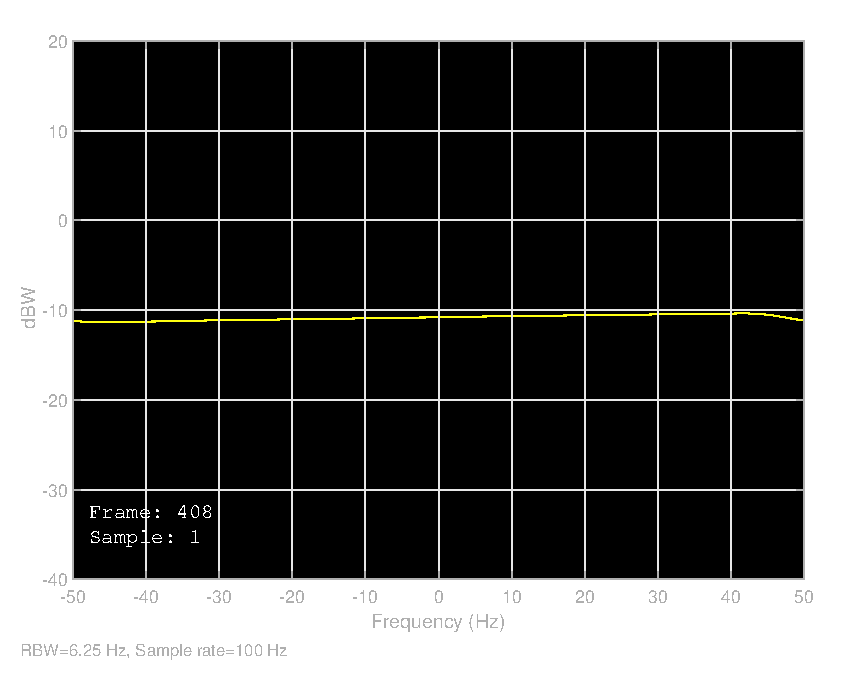
\includegraphics[width=\textwidth]{FrequencyResponse}
			\caption{Figure showing the frequency response of the model}
			\label{fig:FreqResponse}
		\end{figure}
		\begin{figure}
			\centering
			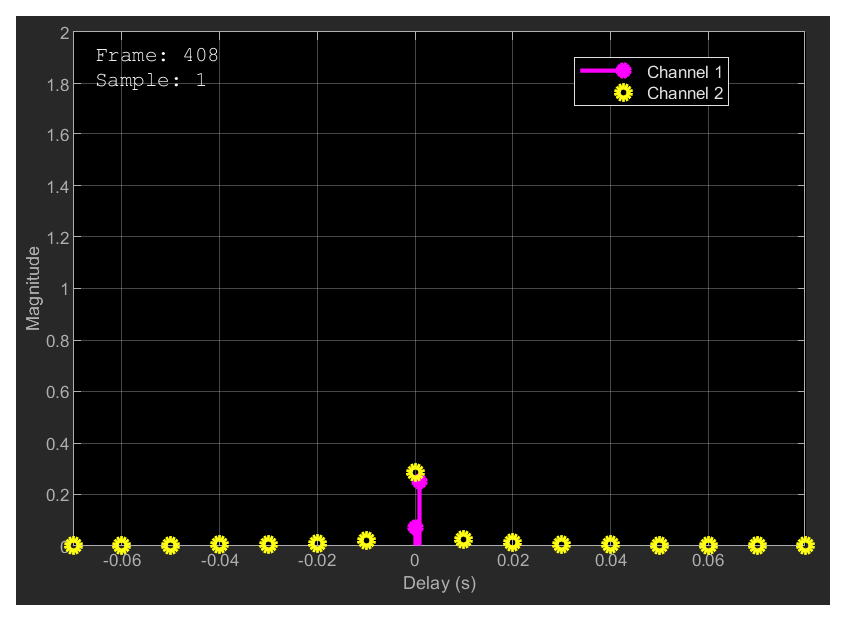
\includegraphics[width=\textwidth]{ImpulseResponse}
			\caption{Figure showing the impulse response of the model}
			\label{fig:ImplResponse}
		\end{figure}
		\Cref{fig:FreqResponse} and \Cref{fig:ImplResponse} show the outputs from the model. These shows that this is a flat fading model. We can prove this mathematically by showing that $B_S << B_C$ and $T_S >> \sigma_\tau$. $B_S$ is represented by the signal bandwidth which is the inverse of
	}
	\section{Conclusion}
	{
		
	}
	
	
	\newpage
	
	\printbibliography[heading=bibintoc,title=References]
\end{document}
